% !TEX encoding = UTF-8
% !TEX TS-program = pdflatex
% !TEX root = ../tesi.tex
% !TEX spellcheck = it-IT

%**************************************************************
\chapter{Il contesto aziendale}
\label{cap:contesto-aziendale}
%**************************************************************

%**************************************************************
\section{H-FARM}

H-FARM nasce nel 2005 con l'obiettivo di aiutare i giovani imprenditori a lanciare le loro idee innovative e supportare la trasformazione delle aziende italiane in un'ottica digitale, il tutto ospitato in un'area verde di 90.000 $ m^2 $ all'interno del parco naturale del fiume Sile.
\\ \\ 
Il 13 Novembre 2015 H-FARM viene ammessa in Borsa, all'interno del segmento AIM (Alternative Investment Market).
\\ \\
Oggi H-FARM è una piattaforma innovativa che:
\begin{itemize}
	\item Sostiene la creazione di nuovi modelli d'impresa attraverso investimenti in \gls{startupg}\glsfirstoccur;
	\item Guida la trasformazione delle grandi aziende verso il digitale;
	\item Fornisce istruzione di alto livello nelle aree del digitale a studenti e professionisti.
\end{itemize}

Il modello d'impresa di H-FARM si basa su tre pilastri fortemente interconnessi tra loro: \textbf{investimento}, \textbf{industria} ed \textbf{istruzione}.

\begin{figure}[htbp]
\begin{center}

\includegraphics[height=2cm]{logos/hfarm_logo}
\caption{Logo H-FARM}
\end{center}
\end{figure}

\subsection{Primo pilastro: investimento}

La chiave per sviluppare una visione d'investimento più ampia e creare nuovi progetti innovativi è il cambiamento. Vengono quindi prese in considerazione idee provenienti da tutta Europa, selezionando quelle più promettenti ed investendo su di esse.
\\ \\
La strategia d'investimento prevede:
\begin{itemize}
	\item Investimenti diretti (da 100.000 \euro{} a 500.000 \euro) in \gls{startupg}\glsfirstoccur{} italiane alle prime armi che abbiano ambizioni nazionali o globali nei campi SaaS e \gls{b2bg}\glsfirstoccur;
	\item Investimenti strategici in \textit{InReach Ventures}: piattaforma di investimento che permette di accedere al fiorente ecosistema delle \gls{startupg}\glsfirstoccur{} presenti in Europa. Ha sede a Londra ed è specializzata \gls{earlystageg}\glsfirstoccur{} nel settore software;
	\item H-CAMP: programma di accelerazione della durata di 4 mesi che mira a sostenere giovani talenti nello sviluppo dei loro modelli d'impresa.
\end{itemize}

L'obiettivo principale è quello di scoprire ed investire nelle \gls{startupg}\glsfirstoccur{} che si concentrano sulle eccellenze italiane: moda e design, cibo e vino, \gls{iotg}\glsfirstoccur, viaggi e turismo.

\subsubsection{H-CAMP}
H-CAMP è un programma di accelerazione internazionale e “all-inclusive”, dedicato a quei talenti ed imprenditori che vogliono sviluppare le proprie idee.
Ogni anno vengono lanciate due \textit{call for ideas}: intervalli temporali entro i quali chiunque può fare domanda per partecipare ad H-CAMP.
\\ \\
H-CAMP fa parte del \textit{Global Accelerator Network}, un'organizzazione internazionale che include tutti i più importanti acceleratori a livello mondiale. Questo permette alle \gls{startupg}\glsfirstoccur{} che entrano a far parte di H-CAMP di poter accedere ad una serie di agevolazioni che vanno dal \gls{mentoring}\glsfirstoccur{} alle relazioni con investitori internazionali.
\\ \\
Il programma è strutturato in 3 fasi, gestite da persone responsabili con competenze tali da poter garantire i migliori risultati ad ogni fase:
\begin{enumerate}
\item \textbf{Selezione delle \gls{startupg}\glsfirstoccur}: vengono scelti i progetti ritenuti più meritevoli tra quelli che hanno risposto alla call for ideas;
\item \textbf{Programma di accelerazione}: la fase di accelerazione è il cuore pulsante del progetto H-CAMP. In questa fase le \gls{startupg}\glsfirstoccur{} selezionate lavorano a stretto contatto con un team di \gls{mentor}\glsfirstoccur{}  ed esperti per sviluppare e consolidare la loro idea d'impresa. Durante questa fase, inoltre, ogni \gls{startupg}\glsfirstoccur{} riceve 20.000 \euro{} per coprire le proprie spese iniziali;
\item \textbf{Demo day}: evento conclusivo del periodo di accelerazione durante il quale le \gls{startupg}\glsfirstoccur{} accelerate presentano il proprio prodotto ad una platea di investitori, aziende, giornalisti e azionisti di H-FARM.
\end{enumerate}

\begin{figure}[htbp]
\begin{center}
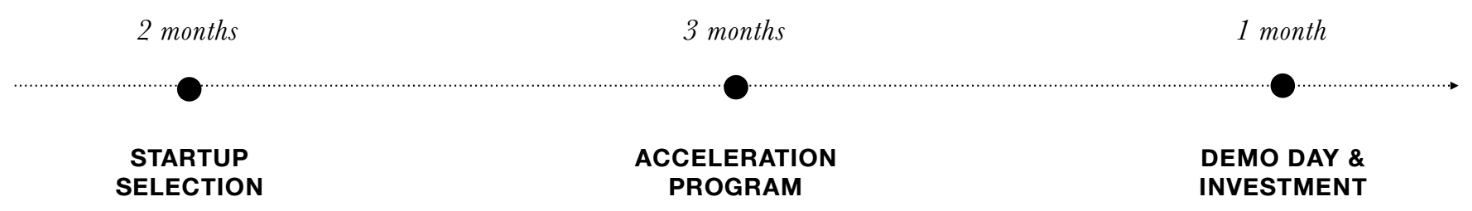
\includegraphics[height=2cm]{hcamp_resume}
\caption{Distribuzione temporale delle fasi previste dal programma H-CAMP}
\end{center}
\end{figure}

\subsection{Secondo pilastro: industria}
Le nuove tendenze tecnologiche dei consumatori obbligano le aziende a rivalutare le modalità con le quali investono sul personale, sui processi e sulle tecnologie. H-FARM aiuta la aziende a trasformare i loro modelli d'impresa e le loro attività in armonia con i cambiamenti digitali in atto.
\\ \\
La strategia per l’industria propone:
\begin{itemize}
\item \textbf{Digital transformation}: formazione, innovazione e rinnovamento dei processi organizzativi per diventare protagonisti del cambiamento digitale in ambito aziendale;
\item \textbf{H-ACK}: maratone di 24 ore focalizzate su specifici settori dell'industria. I partecipanti si dividono in team e lavorano per trovare soluzioni a problemi concreti esposti dalla compagnia promotrice dell'evento.
\end{itemize}

\subsection{Terzo pilastro: istruzione}
I tradizionali sistemi educativi stanno rapidamente diventando obsoleti e la domanda di metodi di apprendimento innovativi è in rapida crescita. H-FARM è il più grande ecosistema digitale attualmente presente in Italia, che unisce le best practice del mondo accademico con nuovi metodi di apprendimento presi in prestito dal mondo del business e delle \gls{startupg}\glsfirstoccur.
\\ \\
Per Maggio 2017 è prevista l'inaugurazione di una nuova area dedicata ad H-CAMPUS: il nuovo progetto formativo di H-FARM dedicato alla diffusione della cultura digitale attraverso un approccio innovativo. 
Studenti, professionisti e manager saranno accompagnati e resi protagonisti del processo di trasformazione digitale.
H-CAMPUS nascerà all'interno di un grande spazio aperto che andrà ad ospitare una \gls{internationalschool}\glsfirstoccur{} (dai 6 ai 18 anni) ed una università con più di 20 tra insegnanti e formatori.

\begin{figure}[htbp]
\begin{center}
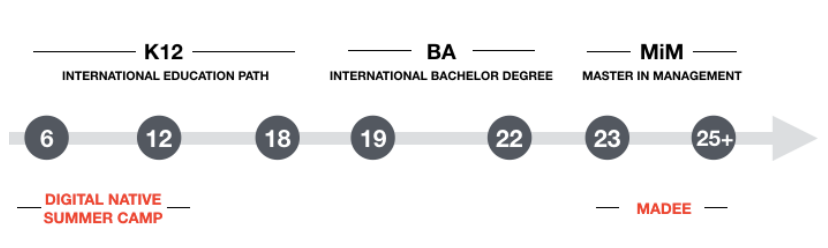
\includegraphics[height=4cm]{hfarm_education_graph}
\caption{Programma H-CAMPUS rivolto a diverse fasce d'età}
\end{center}
\end{figure}

%**************************************************************
\section{Digital Accademia}
Digital Accademia è il centro italiano di riferimento per la diffusione della cultura digitale ed è  situata all'interno dell'ecosistema H-FARM. \\
Questo è il luogo dove studenti, professionisti e innovatori possono conoscere il potenziale del digitale, integrarlo nei propri processi di sviluppo e guardare al futuro. Il tutto viene veicolato attraverso un approccio concreto, con il quale si mira alla formazione attraverso l'esperienza.
\\ \\
L'offerta di Digital Accademia si rivolge principalmente alle aziende e propone strumenti di gestione della conoscenza, strumenti di comunicazione e sessioni formative che consentano di rimanere al passo con il cambiamento costante. La cultura digitale offre possibilità di interazione impensabili fino a poco tempo fa e permette di veicolare contenuti in modo nuovo, coinvolgente, personale e non convenzionale.

\begin{figure}[htbp]
\begin{center}

\includegraphics[height=3cm]{logos/da_logo}
\caption{Logo Digital Accademia}
\end{center}
\end{figure}

\subsection{Formazione}
Diffondere la cultura digitale in azienda significa prima di tutto venire in contatto con le persone e con le loro competenze. L'innovazione del digitale non è un concetto astratto
ma una prassi, per questo non bastano corsi di aggiornamento o sessioni di formazione in aula. 
La formazione deve essere, prima di tutto, un'esperienza che coinvolge. 

\subsubsection{Bootcamp}
All'interno dell'offerta di formazione si colloca il progetto \textbf{Bootcamp}: un'esperienza full immersion di 3 giorni e 3 notti sulla cultura digitale, ospitata in Villa Annia: il quartier generale di Digital Accademia.
\\ \\
Le giornate alternano momenti di teoria a sessioni di pura pratica, mentre i pranzi, le cene e le sere sono momenti sempre conviviali arricchiti dalla presenza di ospiti ed esperti del settore di pertinenza per: 
\begin{itemize}
\item Imparare a pensare digitale;
\item Capire come funziona una buona storia;
\item Scoprire le logiche dietro a un e-commerce di successo; 
\item Costruire presentazioni persuasive.
\end{itemize}

\subsection{Comunicazione interna}
Le esperienze di comunicazione interna più efficaci parlano ai dipendenti come si parlerebbe al pubblico di un evento di \textit{entertainment}. 
L’avvento massiccio del digitale ha fatto sì che non ci sia più differenza tra comunicazione esterna ed interna all’azienda.

\subsubsection{Plot}
All'interno dell'offerta per la comunicazione interna si colloca il progetto \textbf{Plot}.
\\ \\
Questo progetto si basa sui principi degli \gls{arg}\glsfirstoccur{} per coinvolgere e divertire le persone all'interno di una organizzazione. I dipendenti si trasformano in giocatori e partecipano alla risoluzione di enigmi come in un romanzo giallo interattivo: analizzando i file aziendali e individuando informazioni nel mondo reale devono riuscire ad arrivare alla soluzione.
\\ \\
Pensato inizialmente per Vodafone, Plot è un'esperienza avvincente progettata per coinvolgere gli impiegati di tutto il mondo in un gioco mirato a salvare una loro collega, Sugita, rapita da un'intelligenza artificiale da essa stessa progettata.
\\ \\
Sugita rivela ai partecipanti di aver lasciato alcune \textit{backdoor} durante la fase di testing dell'intelligenza artificiale, ogni backdoor richiede una password che può essere trovata da qualche parte all'interno della intranet Vodafone. 
Per trovare le password, i giocatori (divisi in gruppi) devono studiare prodotti specifici dell'azienda, guardare tutorial e interagire tra loro e con i sistemi interni.
\\ \\
Sono previsti dieci livelli e dieci settimane di gioco, durante le quali i team provenienti da tutto il mondo si sfidano per salvare Sugita.
\\ \\
Terminati i dieci livelli, è prevista un'ultima fase nella quale le migliori squadre da tutto il mondo si sfidano a Londra in un'intensa giornata di gioco.
\\ \\
La squadra vincitrice si aggiudica le 6.000 sterline messe in palio come ricompensa.
\\ \\
Il Plot sviluppato per Vodafone ha registrato un grande successo, con oltre 8.000 giocatori distribuiti in 21 paesi. Questo ha portato a riproporre il format per altri clienti, tra i quali TUI Group e Assicurazioni Generali. 

\paragraph{La struttura}
\label{par:struttura-plot}
Perchè abbia successo, il gioco non deve essere presentato come tale ma deve confondersi quanto più possibile con la realtà degli eventi. A questo scopo, la presentazione deve avvenire all'interno del contesto lavorativo. Ad esempio, nel caso di Vodafone, il meeting annuale dei dipendenti veniva interrotto da un video nel quale l'intelligenza artificiale comunicava di aver rapito Sugita e sfidava i colleghi a salvarla.
\\ \\
Dopo aver effettuato la registrazione presso il sistema, la piattaforma prevede una \textbf{fase di inviti} durante la quale ogni utente può invitare un certo numero di colleghi a far parte della propria squadra.
\\ \\
Al termine di questa fase, un algoritmo si occupa di formare le squadre secondo le preferenze espresse dagli utenti. Idealmente, se l'utente A sceglie l’utente B e l’utente B accetta, gli utenti A e B vengono inseriti nella stessa squadra.
\\ \\
Una volta chiusa la fase di inviti e formate le squadre, inizia la \textbf{fase di gioco}. 
La fase di gioco si articola in varie \textbf{mission}, ognuna può essere pensata come un blog che, durante la settimana, viene popolato tramite \textbf{post} appartenenti a tre possibili tipologie: 
\begin{itemize}
	\item \textbf{Testo}: introduce, in modo molto generale, l’obiettivo della mission e può avere contenuti multimediali come immagini e video;
	\item \textbf{Captcha}: prevede una domanda rivolta singolarmente all'utente, atta a verificare che esso sia effettivamente un umano e non una macchina;
	\item \textbf{Team}: prevede una domanda rivolta alla squadra. 
\end{itemize}

In questa fase, ogni settimana prevede due momenti chiave:
\begin{itemize}
	\item Ogni \textbf{lunedì} viene pubblicata una nuova mission, alla quale sono associati inizialmente un post di tipo testo e un post di tipo captcha;
	\item Ogni \textbf{mercoledì} viene pubblicato un post di tipo team, associato alla mission del lunedì.
\end{itemize}

\begin{figure}[htbp]
\begin{center}
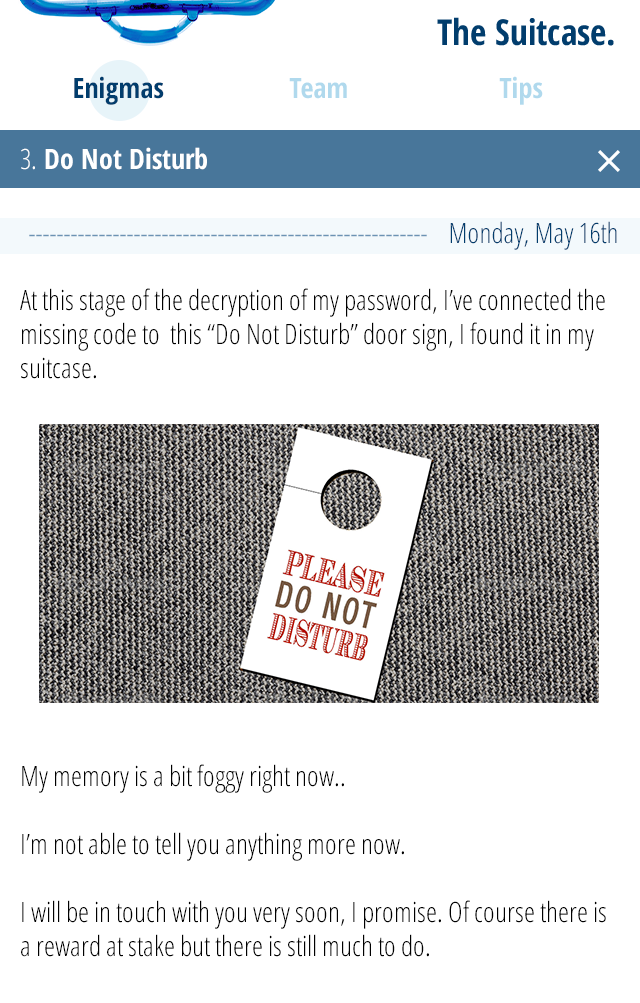
\includegraphics[height=9cm]{plot/text_post}
\caption{Un post di tipo testo}
\end{center}
\end{figure}

\begin{figure}[htbp]
\begin{center}
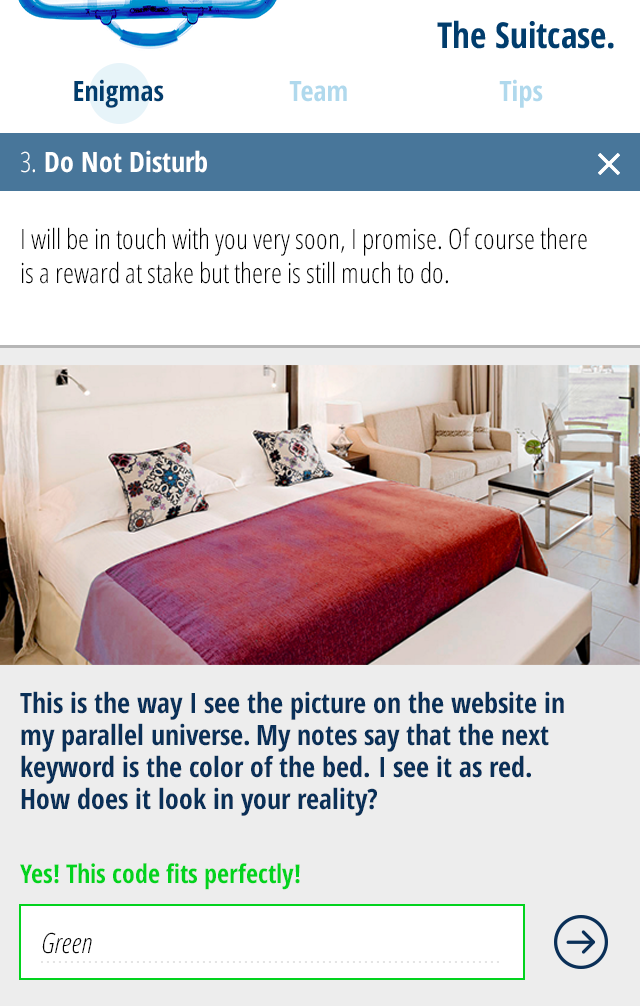
\includegraphics[height=9cm]{plot/captcha_post}
\caption{Un post di tipo captcha}
\end{center}
\end{figure}

\begin{figure}[htbp]
\begin{center}
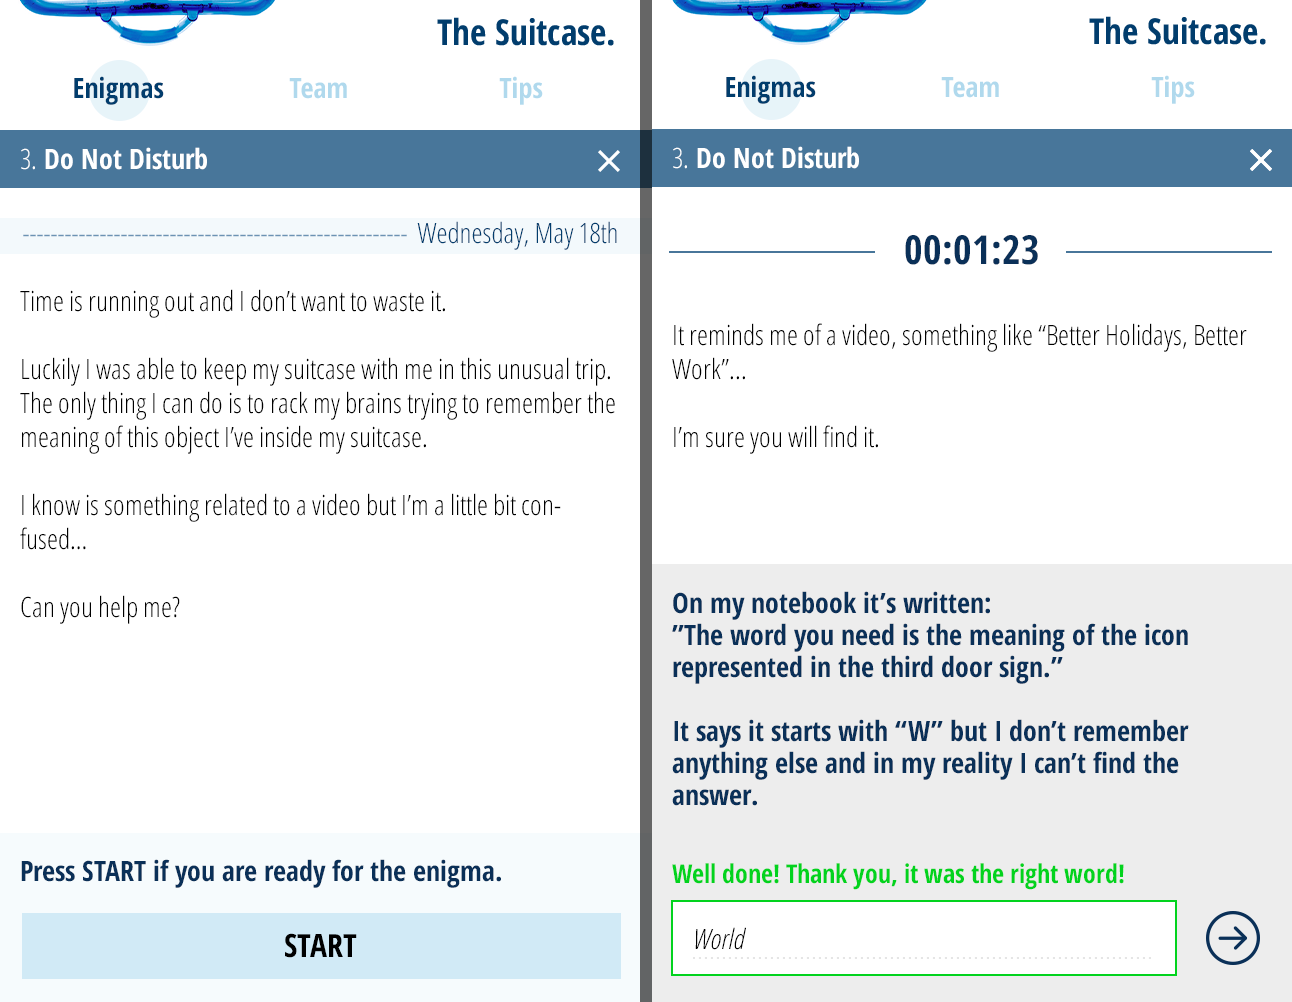
\includegraphics[height=9cm]{plot/team_post}
\caption{Un post di tipo team}
\end{center}
\end{figure}

Per accedere al post di tipo team è necessario che almeno la metà dei componenti della squadra abbia risposto alla propria domanda di tipo captcha. 
\\ \\
Le domande di tipo captcha sono uniche rispetto all'utente e alla squadra, con questo si intende che una specifica domanda di tipo captcha:
\begin{itemize}
	\item non viene presentata allo stesso utente più di una volta;
	\item non viene presentata ai compagni di squadra.
\end{itemize}

La domanda associata al post di tipo team non è immediatamente visibile alla pubblicazione del post, ma può essere svelata da un componente della squadra. Una volta svelata la domanda di tipo team, viene avviato un cronometro che registra il tempo impiegato dalla squadra per rispondere.
\\ \\
Mentre le domande di tipo captcha sono pensate per richiedere uno sforzo minimo all’utente, quelle di tipo team hanno grado di difficoltà più alto, che aumenta col progredire del gioco.
\\ \\
Le domande sono pensate in modo da portare gli utenti ad affrontare specifici \textbf{touchpoint}: strumenti o concetti che l'azienda vuole far conoscere ai propri dipendenti. \\
Ad esempio, nel caso di Vodafone, Plot è stato progettato per perseguire i seguenti touchpoint:
\begin{itemize}
	\item Far conoscere ai dipendenti di tutto il mondo una nuova area della intranet aziendale;
	\item Creare coesione tra i dipendenti;
	\item Attivare forme di coinvolgimento dirette attraverso la costruzione di un'esperienza;
	\item Trovare nuovi strumenti globali di comunicazione interna.
\end{itemize}

La squadra riceve un punteggio per ogni mission e, tale punteggio, è una funzione del tempo impiegato per rispondere alla domanda di tipo team. \\
Il punteggio totale di una squadra, che determina la posizione in classifica della stessa, è ricavato come somma dei punteggi ottenuti nelle varie mission.
